\thispagestyle{cackithitoannone}
\pagestyle{cackithitoan}
\everymath{\color{cackithi}}
\graphicspath{{../cackithi/pic/}}
\begingroup
\AddToShipoutPicture*{\put(0,616){
\includegraphics[width=19.3cm]{../bannercackithi}}}
\AddToShipoutPicture*{\put(152,570){
\includegraphics[scale=1]{../tieude1.pdf}}}
\centering
\endgroup
\vspace*{140pt}

\begin{multicols}{2}
	Trong phần đầu chuyên mục, chúng tôi sẽ trình bày với các bạn lời giải của các bài toán trong Kỳ thi Olympic Toán học Quốc gia Israel năm $2023$, đăng trong số báo $12/2023$. 
	\begin{figure}[H]
		\vspace*{-5pt}
		\centering
		\captionsetup{labelformat= empty, justification=centering}
		
\includegraphics[width= 0.85\linewidth]{gocolympic}
		%		\caption{\small\textit{\color{}}}
		\vspace*{-5pt}
	\end{figure}
	{\bf\color{cackithi} OC$\pmb{58.}$} Có $2000$ người ngồi quanh một chiếc bàn tròn. Mỗi người trong số họ là người  thật thà (người luôn nói thật) hoặc kẻ  dối trá (người luôn nói dối). Biết rằng mỗi người đều nói: ``Ít nhất hai trong số ba người ngồi ngay sát bên phải của tôi là những kẻ dối trá". Hỏi có bao nhiêu người thật thà ngồi trong bàn?
	\vskip 0.1cm
	\textit{Lời giải.} Ta nhận xét rằng nếu có $2$ người thật thà $A, B$ ngồi cạnh nhau lần lượt theo chiều kim đồng hồ thì $2$ người ngồi tiếp theo theo $C, D$ đều là dối trá vì $A$  nói thật. Hơn nữa do $C$ nói dối nên cả hai người tiếp theo đều là thật thà. Cứ tiếp tục lý luận như vậy ta thấy rằng những người này ngồi xen kẽ nhau: $2$ người thật thà liên tiếp, rồi lại $2$ người dối trá, rồi lại $2$ người thật thà ... Như vậy trong trường hợp này có đúng $1000$ người thật thà. Trường hợp có hai người dối trá ngồi cạnh nhau ta cũng lý luận tương tự và nhận được cùng một kết quả.
	\vskip 0.1cm
	Trường hợp không có $2$ người cùng thật thà hay cùng dối trá ngồi cạnh nhau thì những người thật thà và dối trá ngồi xen kẽ. Ta thấy cách ngồi này cũng thỏa mãn đầu bài. Như vậy trong mọi trường hợp luôn có đúng $1000$ người thật thà.   
	\vskip 0.1cm
	{\bf\color{cackithi} OC$\pmb{59.}$} Biết rằng các số nguyên không âm $x,y$ thỏa mãn
	\begin{align*}
		\sqrt{x}+\sqrt{x+60}=\sqrt{y}.
	\end{align*}
	Tìm giá trị lớn nhất có thể của $x$.
	\vskip 0.1cm
	\textit{Lời giải.}
	Bình phương  hai vế ta thu được $2x+60+2\sqrt{x^2+60x}=y.$ Do đó ${x^2+60x}$ phải là một số chính phương. Đặt $x^2+60x=m^2,$ với $m$ nguyên dương, ta nhận được
	\begin{align*}
		(x+30)^2-m^2&=(x+30+m)(x+30-m)\\
		&=900.
	\end{align*}
	Như vậy nếu đặt $u=x+30+m, v=x+30-m$ thì  ta có $uv=900$ và $ x=\frac{u+v}{2}-30.$  Ta thấy $x$ đạt giá trị lớn nhất khi $u+v$ đạt giá trị lớn nhất. Hơn nữa, do $(u+v)^2=(u-v)^2+4uv= (u-v)^2+ 3600$ đạt giá trị  lớn nhất khi chênh lệch giữa $u$ và $v$ lớn nhất. Chú ý rằng $u-v=2m$ nên $u, v$ cùng tính chẵn lẻ và trường hợp $u=900, v=1$ không xảy ra. Vậy $u+v$ đạt giá trị lớn nhất khi $u=450, v=2.$ Khi đó ta giải được $m=224$ và $x=196.$ Vậy giá trị lớn nhất có thể của $x$ là $196$.
	\vskip 0.1cm
	{\bf\color{cackithi} OC$\pmb{60.}$} Liệu có tồn tại một tập hợp $S$ gồm $5783$ số thực phân biệt thỏa mãn điều kiện sau hay không:
	Với mọi $a,b\in S$ (không nhất thiết phải phân biệt) đều tồn tại hai số $c\neq d$ thuộc $S$ sao cho $a \times b=c+d$?
	\vskip 0.1cm
	\textit{Lời giải.} Ta xét phương trình $f(x)=x^{2891}-x-1=0.$ Do $f(1)=-1<0, f(2)=2^{2891}-3>0$ nên tồn tại giá trị $z\in (1,2)$ để $f(z)=0.$ 
	\vskip 0.1cm
	Ta chọn tập $S=\{0, \pm 1, \pm z, \cdots, \pm z^{2890}\}.$ Khi đó nếu $a,b\in S$ mà $ab=0$ thì ta chọn $c=1, d=-1.$ Trường hợp $ab\neq 0$ thì $ab=\pm z^k$ với $0\le k \le 5780.$ Ta xét hai trường hợp:
	\vskip 0.1cm
	Trường hợp $1$: $0\le k \le 2890.$ Ta chọn $c=\pm z^k$ và $d=0$.
	\vskip 0.1cm
	Trường hợp $2$: $2891\le k \le 5780.$ Do $z^{k}=z^{k-2891}z^{2891}=z^{k-2891}(z+1)=z^{k-2890} +z^{k-2891}.$ Ta chọn $c=\pm z^{k-2890}, d=\pm z^{k-2891}.$
	\vskip 0.1cm
	Như vậy tập $S$ thỏa mãn điều kiện trong bài toán.
	\vskip 0.1cm
	Trong phần cuối của chuyên mục kỳ này, chúng tôi sẽ giới thiệu với bạn đọc ba bài toán trong Kỳ thi Toán Harvard--MIT $2/2024$. Đây là cuộc thi dành cho học sinh trung học do các sinh viên từ hai trường đại học Harvard và MIT tổ chức. Các bài toán sau phù hợp với học sinh lớp $8-10$. 
	\vskip 0.1cm
	{\bf\color{cackithi} OC$\pmb{67.}$} Cho $ABCD$ là hình vuông và $\ell$ là đường thẳng đi qua trung điểm của đoạn $AB$ và cắt  đoạn $BC$. Cho khoảng cách từ $A$ và $C$ đến $\ell$ lần lượt là $4$ và $7$, hãy tính diện tích của $ABCD.$
	\vskip 0.1cm
	{\bf\color{cackithi} OC$\pmb{68.}$} Tính tổng của tất cả các số nguyên dương $n$ thỏa mãn $50 \le n \le 100$ và $2n + 3$ không là ước của $2^{n!} -1.$
	\vskip 0.1cm
	{\bf\color{cackithi} OC$\pmb{69.}$} Một con ốc sên bò trong các ô của một bảng ô vuông cỡ $3\times 24$ ($3$ hàng và $24$ cột) như hình vẽ minh họa. Mỗi lần ốc sên đi từ ô hiện tại đến một ô kề bên có chung cạnh và muốn đi qua tất cả các ô của bảng, mỗi ô đúng $1$ lần. Giả sử ốc sên xuất phát từ ô ở hàng thứ $2$ cột thứ nhất như trong hình, hỏi có bao nhiêu đường đi khác nhau mà ốc sên có thể đi.
	\begin{figure}[H]
		\vspace*{-5pt}
		\centering
		\captionsetup{labelformat= empty, justification=centering}
		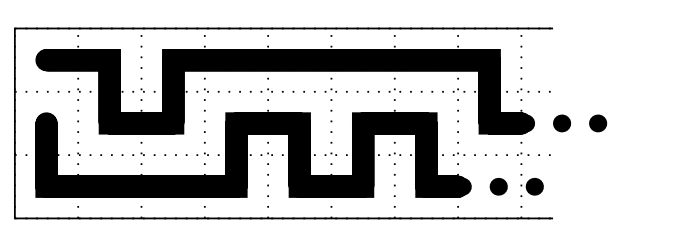
\includegraphics[width= 1\linewidth]{OC69}
%		\caption{\small\textit{\color{}}}
		\vspace*{-10pt}
	\end{figure}	
\end{multicols}
